\documentclass[conference]{IEEEtran}
\IEEEoverridecommandlockouts
% The preceding line is only needed to identify funding in the first footnote. If that is unneeded, please comment it out.
\usepackage{cite}
\usepackage{amsmath,amssymb,amsfonts}
\usepackage{algorithmic}
\usepackage{graphicx}
\usepackage{textcomp}
\usepackage{xcolor}
\usepackage{url}
\def\BibTeX{{\rm B\kern-.05em{\sc i\kern-.025em b}\kern-.08em
    T\kern-.1667em\lower.7ex\hbox{E}\kern-.125emX}}
\begin{document}

\title{BlockID}

\author{\IEEEauthorblockN{1\textsuperscript{st} Given Name Surname}
\IEEEauthorblockA{\textit{dept. name of organization (of Aff.)} \\
\textit{name of organization (of Aff.)}\\
City, Country \\
email address or ORCID}
\and
\IEEEauthorblockN{2\textsuperscript{nd} Given Name Surname}
\IEEEauthorblockA{\textit{dept. name of organization (of Aff.)} \\
\textit{name of organization (of Aff.)}\\
City, Country \\
email address or ORCID}
}

\maketitle

\begin{abstract}
This is technical document for our final blockchain project. Which is about a D-Application where users can use NFTs as a form of digital profile verification.
\end{abstract}

\begin{IEEEkeywords}
Decentraliez application, blockchain, Know Your Customer, Non Fungible Token
\end{IEEEkeywords}

\section{Introduction}
In Know Your Customer (KYC) processes, many companies are required by law to collect and store users’ personal data for verification. This includes the user’s name and phone numbers, home and email addresses, passport images and other forms of photo ID.

These types of processes are prevalent on the internet, and users often must manually enter their personal information into individual online forms. This is not only tedious, but also creates unnecessary privacy risks. In addition to being stored on a centralized server, personal data is vulnerable to spyware and phishing attempts during the process of sharing it.

We provide a new solution for this problem by proposed a block chain based application with Non Fungible Token (NFT)

\section{Approach}

\subsection{Requirement}
The system mints an NFT after the user submits a mint request with the relevant document(s).

The system sends an NFT via a smart contract after the user submits a transaction request with a wallet address.

The system displays all user NFTs after the user submits a request to view all their NFTs

The user is able to interact with the system through an easy-to-use interface

\subsection{Tech used}
MetaMask: MetaMask is a software cryptocurrency wallet that is used to interact with the Ethereum chain and is one of the most popular wallets that we can use.

Web3js(NodeJS): Web3JS is a popular library that basically encodes and decodes any data prior to, or after interaction with the blockchain. It is used to interact with local or remote Ethereum nodes using HTTP, IPC or WebSocket. 

Remix IDE: Remix IDE as a no-setup tool with a web user interface to develop and interact with smart contracts.

Ethereum: Most common for D-apps development due to its high transaction speed, high security and smart contract support. 

Geth: Used to create and host the private Ethereum blockchain network.

IPFS - a peer-to-peer file storing and sharing distributed system.

Front-end: Develop interactive front-end for users with simple React, JavaScript, HTML and CSS.

\subsection{Programming language}
Solidity: Used to develop smart contracts on the Remix IDE, which will be deployed to the Ethereum private network.

React, JavaScript, HTML, CSS: Used to make an interactive and user-friendly webpage as the frontend of the D-application.


\section{Architechture}
\subsection{Blockchain}
The private blockchain is built based on Ethereum using Geth. We create and mine our own blocks. The blockchain have full functionality of Ethereum and providing multiple interfaces.
After creating blockchain, we can set up new account and connect to Metamask wallet. Then we can mine and use Remix IDE for testing smart contract.
\begin{figure}[ht]
\centerline{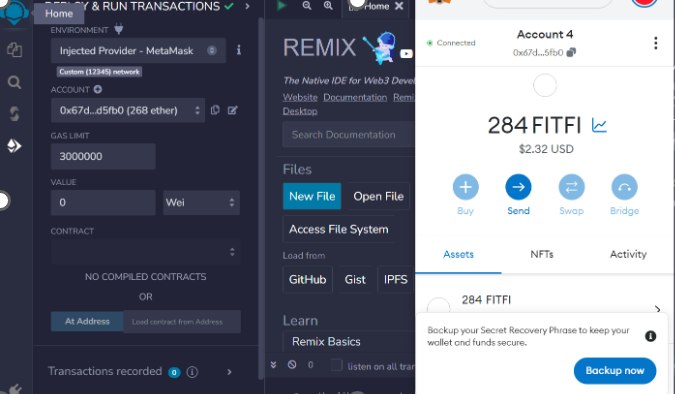
\includegraphics[width=0.45\textwidth]{Etherium.png}}
\caption{Working Private Etherium network and connect to MetaMask}
\label{fig1}
\end{figure}


\subsection{Smart contract and NFT}
User sends NFT mint request to admin for approval
\begin{enumerate}
  \item User sends an NFT mint request to an admin along with the relevant documents, via a public function.
  \item The admin can view the document and can either reject or approve the request, via a function that requires the admin account to use.
  \item Upon rejection, a notification is sent to the user. (tbd)
  \item Upon approval, an NFT is minted and sent to the user.
The smart contract was first tested on Remix IDE and then deploy to our own network by Truffle. 
The NFT is created based on ERC721 standard and boostrap from a github library. 
\begin{figure}[ht]
\centerline{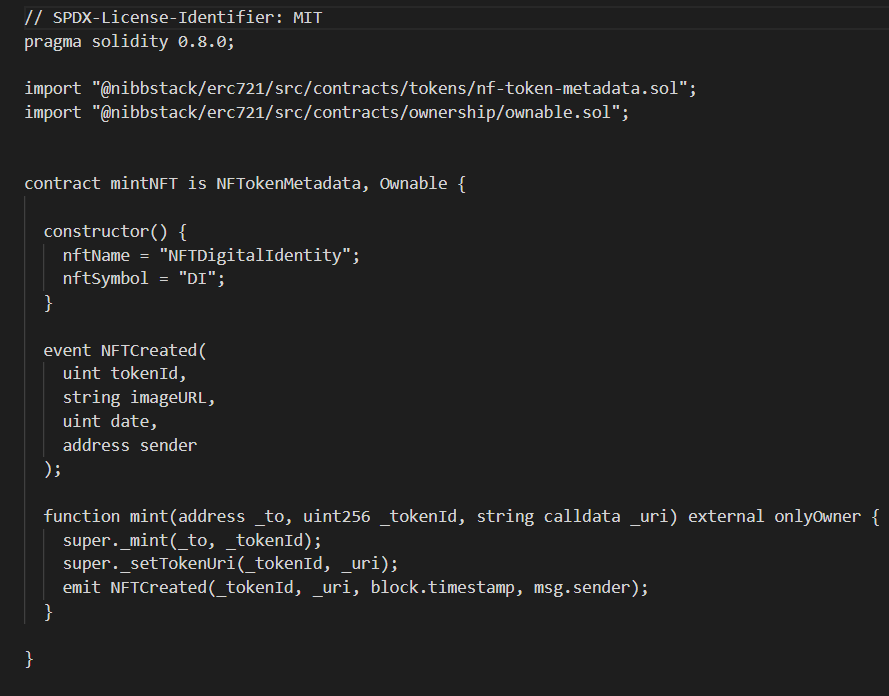
\includegraphics[width=0.45\textwidth]{Smartcontract.png}}
\caption{Our Smart contract}
\label{fig2}
\end{figure}
\end{enumerate}

To handle NFT, user have to upload a image file. Then, we need to host our document for NFT and create a metadata file by using IPFS:
\begin{figure}[ht]
\centerline{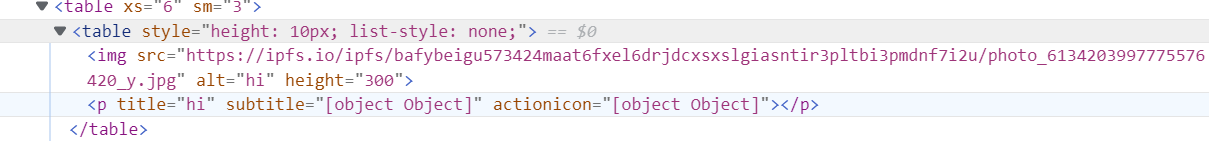
\includegraphics[width=0.45\textwidth]{Ipfs.png}}
\caption{Data handle by IPFS}
\label{fig3}
\end{figure}

\subsection{Front-end}
We use React as our main component for the front end. Blockchain, smart contract connect to front end by Web3js and Metamask.
\begin{figure}[ht]
\centerline{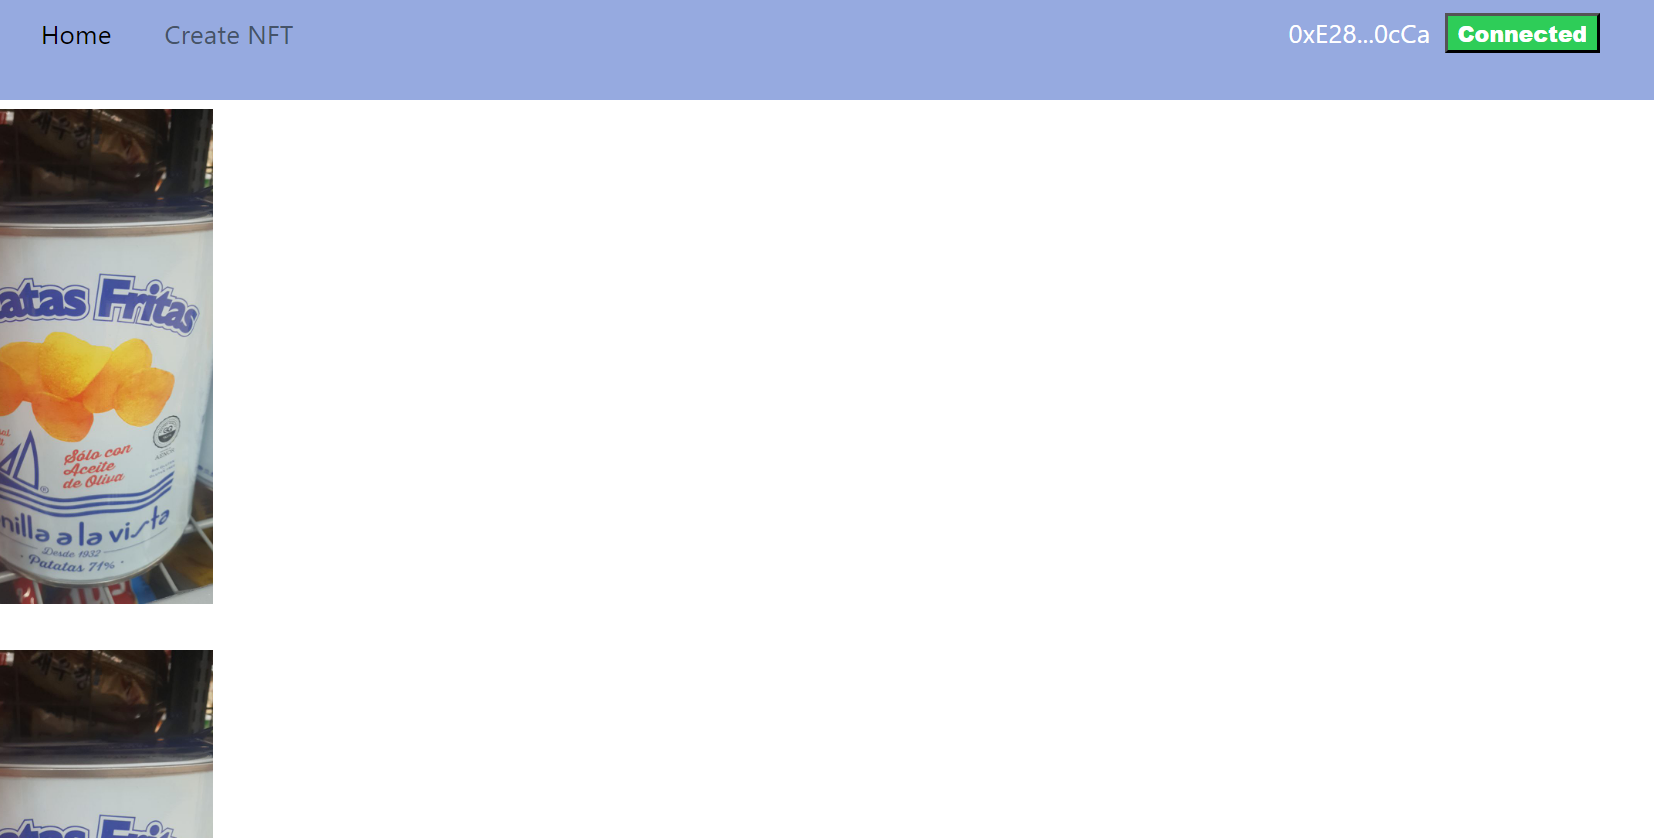
\includegraphics[width=0.45\textwidth]{Front-end.png}}
\caption{Our Front end and it is connected to our network}
\label{fig4}
\end{figure}

\begin{figure}[ht]
\centerline{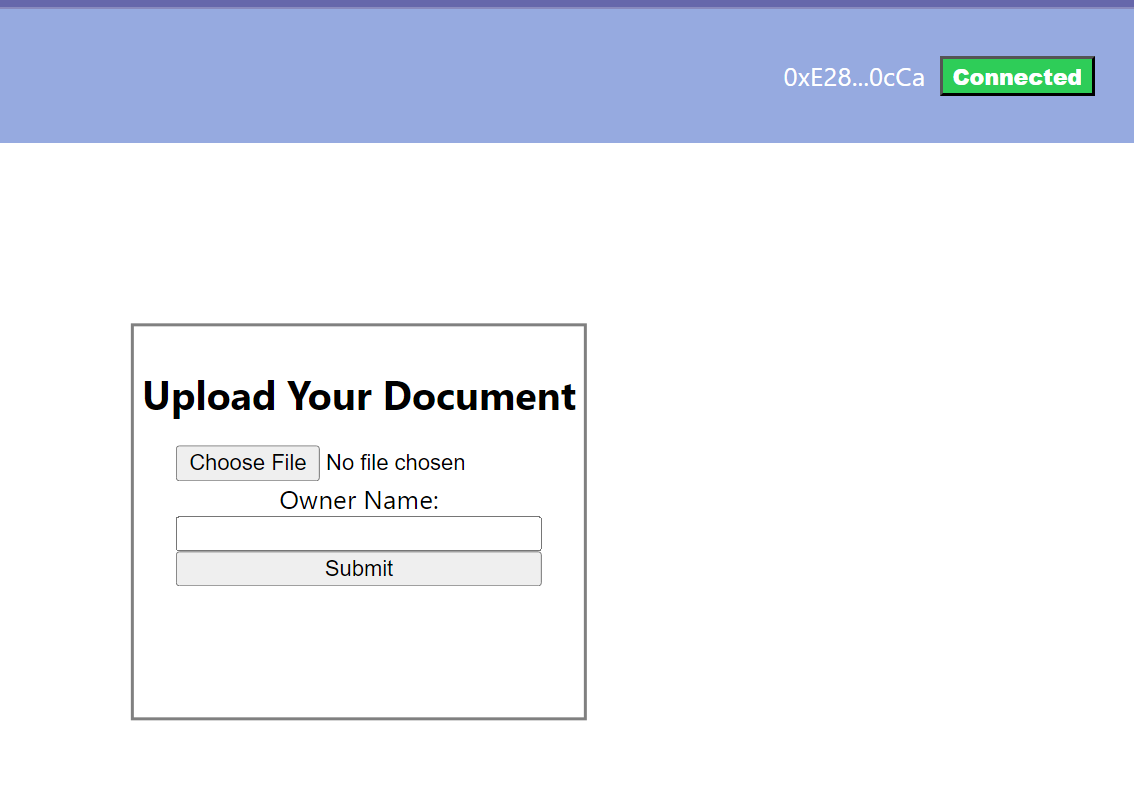
\includegraphics[width=0.45\textwidth]{Upload.png}}
\caption{User upload file after connecting to network}
\label{fig5}
\end{figure}


\subsection{Verification}
After having the NFT, other user can see the NFT in project homepage. The NFT acts as a proof for verification without spending time.  

\section{Deployment}
Download code here.
\begin{enumerate}
    \item Install through git bash with command:
    \begin{itemize}
        \item With npm: "npm install --save --save-exact"
        \item with yarn: "yarn add --exact"
    \end{itemize}
    \item Run your own local etherium blockchain by geth and specify your host, port and address. Change the information accordingly in file "truffle-config.js" and "App.js"
    \item Check the Ipfs API key and change it to your own on "pages/approve-nft.js"
    \item Run the application
        \begin{itemize}
        \item With npm: "npm start"
        \item with yarn: "yarn start"
    \end{itemize}
\end{enumerate}

\section{Related work}

GetID project for online verification in crypto world activities e.g. exchange,... \cite{b1} \cite{b2}. 

\begin{thebibliography}{00}
\bibitem{b1} Identity Verification for Crypto Industry
 \url{https://getid.com/industries/crypto/}, May 2023.
\bibitem{b2} An all-in-one workflow solution to verify  customers’ identities\url{https://kyc-chain.com/}, May 2023.

\end{thebibliography}

\end{document}
